\documentclass[10pt,a4paper]{article}
\usepackage[utf8]{inputenc}
%\usepackage[portuguese]{babel}
\usepackage[T1]{fontenc}
\usepackage{amsmath}
\usepackage{hyperref}
\usepackage{amsfonts}
\usepackage{amssymb}
\usepackage{makeidx}
\usepackage{graphicx}
\usepackage{imakeidx}

\makeindex

\title{Viva Melhor}
\author{Omeir Haroon 61810}
\date{\today}


\begin{document}


\begin{titlepage}
	\begin{center}
	{\Huge\bfseries Viva Melhor}\\
	\vspace{1cm}
	{\Large Engenharia Informática}\\
	\vspace{1cm}
	{\Large Turma 3 (TP 18)}\\
	\end{center}
	\begin{flushright}
	{\Large OMEIR HAROON \Large 61810 \hfill  \large\today}
	\end{flushright}
	\begin{figure}[h]
	\begin{center}
	\scalebox{1}{
\includegraphics{capa_img.PNG}}
	\end{center}
	\end{figure}
\end{titlepage}



\section{Introdução}\index{Introdução}
	Seguro de saúde refere-se a um tipo de "proteção"
que pessoas podem obter para ajudar a pagar por serviços médicos. É i,portante pois quem tem preocupa-se menos com os custos de assistência médica.
\begin{quote}
    "No one plans to get sick or hurt, but most people need medical care at some point. Health insurance covers these costs and offers many other important benefits." \cite{healthcare}
\end{quote}

\begin{table}[h]
	\centering
	\caption{Vantagens e Desvantagens de seguro de saúde}
	\begin{tabular}{|c|c|} 
	\hline
	{\bfseries Vantagens} & {\bfseries Desvantagens}\\
	\hline
	Independência &  Custo\\
	\hline	
	Liberdade de escolha & Exclusões\\
	\hline	
	Tempo de espera  & Franquia\\
	\hline
	\end{tabular}
\end{table}
\newpage

\section{Caso de Estudo}\index{Caso de Estudo}
\begin{quote}
A Declaração Universal dos Direitos Humanos garante saúde e um nível de vida adequado. Em Portugal, o SNS é universal e frequentemente gratuito. Devido à demanda, a iniciativa privada oferece seguros de saúde. Nelson avalia três propostas de uma Companhia de Seguros, a serem registradas na tabela (exemplo: 61810).
\end{quote}

\begin{table}[!ht]
    \centering
    \begin{tabular}{|l|l|l|l|}
    \hline
        ~ & Seguro A & Seguro B & Seguro C \\ \hline
        Anuidade & 81 & 10 & 61 \\ \hline
        Tarifa de ato médico diurno & 9 & 7 & 14\\ \hline
        Tarifa de ato médico noturno & 7 & 0 & 4  \\ \hline
        Atos médicos oferecidos com a anuidade & 10 & 15 & 20 \\ \hline

    \end{tabular}
	\caption{Tabela de preços dos tres tipos de seguros}
	
\end{table}


\begin{table}[!ht]
    \centering
    \begin{tabular}{|l|l|l|l|}
    \hline
        Nº Atos Médicos Anuais & Seguro A & Seguro B & Seguro C \\ \hline
        10 & 0 & 0 & 0\\ \hline
        20 & 82 & 21 & 0  \\ \hline
        30 & 164 & 63 & 100  \\ \hline
        40 & 246 & 105 & 200 \\ \hline
        50 & 328 & 147 & 300 \\ \hline
        60 & 410 & 189 & 400  \\ \hline
        70 & 492 & 231 & 500 \\ \hline
        80 & 574 & 273 & 600 \\ \hline
        90 & 656 & 315 & 700  \\ \hline
    \end{tabular}
	\caption{Comparação dos precos em relação ao numero de atos médicos}
\end{table}

\begin{figure}[!ht]
	\scalebox{1}{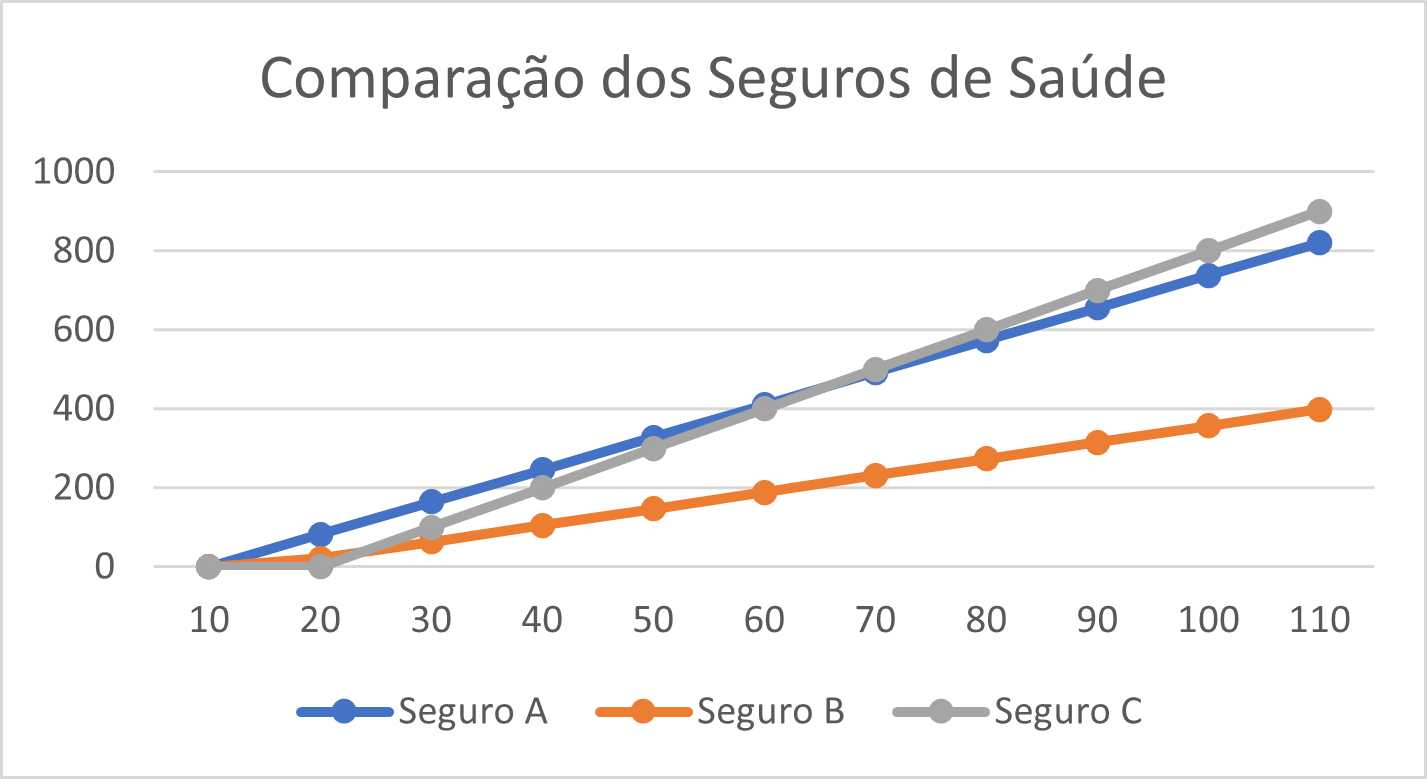
\includegraphics{graph}}
	\caption{Comparação de seguros de saude}
\end{figure}

\newpage
\section{Conclusão}\index{Conclusão}

Após analisar as propostas dos seguros de saúde (A, B, C) para o senhor Nelson, algumas conclusões podem ser destacadas:

1. \textbf{Custo vs. Benefício:} O Seguro B apresenta a menor anuidade e tarifas de atos médicos, tornando-o uma opção mais acessível.

2. \textbf{Cobertura de Atos Médicos:} O Seguro C oferece uma ampla cobertura de atos médicos, especialmente para valores mais altos. Isso pode ser vantajoso para quem espera precisar de cuidados médicos frequentes.

3. \textbf{Liberdade de Escolha:} Todos os seguros oferecem liberdade de escolha, mas o Seguro C pode ser mais atrativo devido à sua cobertura abrangente.

4. \textbf{Ponderação Pessoal:} A escolha entre os seguros deve ser baseada nas necessidades específicas do senhor Nelson e sua família. Se a prevenção e a cobertura abrangente são prioridades, o Seguro C pode ser a melhor opção. Se a preocupação principal é o custo, o Seguro B pode ser mais adequado.

Em última análise, a decisão deve refletir as prioridades pessoais e a situação financeira. Recomenda-se que o senhor Nelson escolha o seguro C se pensa que nao vai precisar mais do 20 atos médicos anuais caso contrario deve escolher o seguro B que é mais barato relativamente.



\section{Bibliografia}\index{Bibliografia}
\begin{thebibliography}{9}
    \bibitem{healthcare}
    HealthCare.gov. "Why Coverage is Important." [Online]
    Available: \url{https://www.healthcare.gov/why-coverage-is-important}
\end{thebibliography}

\printindex

\end{document}